\section{How to Make Lots of Mistakes} 

An important challenge from section~\ref{sec:challenges} is the generation of
mix-typed programs with representative impedance mismatches between
the typed components, their types, and the behavior of untyped components. In this section, we
present a generation process and argue that, despite its synthetic
nature, it yields a large corpus of programs with  realistic and diverse type mistakes.


\begin{figure*}
\begin{tabular}{p{2cm} | p{10cm} }
  {\bf  name} & {\bf description (author)}  \\

\hline

  \texttt{acquire} & Object-oriented board game implementation (M. Felleisen)  \\%[1em]


\hline
  \texttt{gregor} & Utilities for calendar dates (J. Zeppieri) \\%[1em]


\hline
  \texttt{kcfa} & Functional implementation of 2CFA for the lambda calculus (M. Might) \\%[1em]


\hline
  \texttt{quadT} & Converter from S-expression source code to PDF format (M. Butterick)\\%[1em]

\hline
  \texttt{quadU} & Converter from S-expression source code to PDF format  (B. Greenman) \\%[1em]

\hline
  \texttt{snake} & Functional implementation of the  Snake video game (D. Van Horn) \\%[1em]

\hline
  \texttt{suffixtree} & Algorithm for common longest subsequences between strings. (D. Yoo) \\%[1em]

\hline
  \texttt{synth} & Converter of notes and drum beats to WAV (V. St-Amour \& N. Toronto) \\%[1em]

\hline
  \texttt{take5} & Mixin-based card game simulator (M.Felleisen)  \\%[1em]

\hline
  \texttt{tetris} & Functional implementation of Tetris (D. Van Horn) \\%[1em]


\end{tabular}
  \caption{Benchmarks summary.}
  \label{table:benchmark-descriptions}
\end{figure*}


The starting point for our corpus of programs
is~\citet{gtnffvf-jfp-2019}'s gradual typing benchmark suite. The
benchmark suite consists of fully typed correct programs that are written by different authors
and have been used, maintained and evolved by their authors and others over a
number of years.  They range widely in size, complexity, purpose and
features of Typed Racket they employ.  Furthermore the benchmarks use advanced aspects
of Typed Racket's type system such as occurrence
typing~\cite{tf-icfp-2010}, types for mutable and immutable data
structures, polymorphic types, types for first-class classes and objects and types for
Racket's numeric tower~\cite{stathff-padl-12}. Without loss of the diversity of the benchmarks,
we select the ten largest in terms of numbers of components (between 6 and 14 components).
These benchmarks also have the most complex dependency graphs and, hence,
can make the debugging process the hardest for the rational programmer.
The table in figure~\ref{table:benchmark-descriptions} shows our selection
together with a short description for each benchmark.



Of course, the gradual typing benchmarks have no mistakes for the rational
programmer to debug. Therefore, we follow ~\citet{lksfd-popl-2020} and we
inject bugs with mutation
analysis~\cite{jia2011analysis,demillo1978hints,lipton1971fault}.  A
mutation is a local syntactic change of the code of a program that may
produce a bug. Usually, the outcome of mutating a program once, dubbed a
mutant, can be distinguished from the original program with a test case.
The better the test suite of a program, the more mutants it can ``kill.''
Mutants that are hard to ``kill'' usually correspond to subtle programming
errors, and mutation frameworks typically come with standard mutators
carefully designed to create such mutants.

However,  unlike the hard-to-kill mistakes introduced by standard mutators, 
gradual type systems flag mere typos.  Thus, in order to
exercise the rational programmer in the context of gradual typing, 
we need to develop alternative mutators
that are fine-tuned to produce the type-level mistakes gradual type systems 
can detect. Our inspiration is our
more-than-a-decade long experience of making type-level mistakes in Typed
Racket. Some of these mistakes often take non-trivial effort to debug and
have become the seed for our mutators, which we summarize in
figure~\ref{table:mutation-ops}.  For each one, the figure provides a
short description and an example mutation.


Most of our mutators are self-explanatory.
The first twelve apply to most gradually typed languages, including those with classes.
The last four mutators target distinguishing features of Typed Racket.
Specifically, \texttt{arithmetic} may replace a \texttt{+} with a \texttt{-}
in an attempt to change the type of the result of the arithmetic
operation. In Typed Racket, \texttt{+}'s result is a
\texttt{Positive-Integer} when all arguments are
positive integers. However, the result of \texttt{-} is
\texttt{Integer}. In the same spirit, \texttt{boolean} aims to take
advantage of Typed Racket's ``truthiness.'' Finally, \texttt{negate-cond} and \texttt{force-cond}
attempt to confuse occurrence typing.


\begin{figure*}
  \begin{tabular}{p{2.1cm} | p{5cm}  | p{5.5cm} }
    {\bf name} & {\bf description} & {\bf example} \\
\hline




    \texttt{constant}
& Swap a literal constant with another of the same value but different type.
& \texttt{5.6} $\rightarrow$ \texttt{5.6+0.0i} \\
\hline

    \texttt{deletion}
    & Deletes the result expression of a sequence.
    & \texttt{(begin x y z)} $\rightarrow$ \texttt{(begin x y)} \\
\hline

   \texttt{position}
 & Swaps two subexpressions.
  &  \texttt{(f a 42 "b" 0)} $\rightarrow$\texttt{(f a 42 0 "b")} \\
\hline

     \texttt{list}
    & Replaces \texttt{append} with \texttt{cons}.
    &  \begin{tabular}[t]{@{}l}
      \texttt{append} $\rightarrow$ \texttt{cons}
    \end{tabular}\\
\hline

    \texttt{top-level-id}
 & Swaps two identifiers defined in the same module.
 &\texttt{(f x 42)} $\rightarrow$ \texttt{(g x 42)}\\
\hline

    \texttt{imported-id}
 & Swaps two identifiers imported from the same module.
 &\texttt{(f x 42)} $\rightarrow$ \texttt{(g x 42)}\\
\hline

    \texttt{method-id}
 & Swaps two method identifiers.
 &\texttt{(send o f x 42)} $\rightarrow$ \texttt{(send o g x 42)}\\
\hline

    \texttt{field-id}
 & Swaps two field identifiers.
    & \begin{tabular}[t]{@{}l} \texttt{(get-field o f)} $\rightarrow$ \\
        \texttt{(get-field o g)}
      \end{tabular}\\
\hline

     \texttt{class:init}
  & Swaps values of class initializers.
   &  \begin{tabular}[t]{@{}l}
     \texttt{(new c [a 5] [b "hello"])} $\rightarrow$\\
     \texttt{(new c [a "hello"] [b 5])}\\
    \end{tabular}\\
\hline

     \texttt{class:parent}
    & Replaces the parent of classes with \texttt{object\%}.
    &  \begin{tabular}[t]{@{}l}
     \texttt{(class foo\% (super-new))} $\rightarrow$\\
     \texttt{(class object\% (super-new))}\\
    \end{tabular}\\
\hline

     \texttt{class:public}
    & Makes a public method private and vice versa.
    & \begin{tabular}[t]{@{}l}
      \texttt{(class object\%}\\
      \phantom{(d}\texttt{(define/public (m x) x))} $\rightarrow$\\
      \texttt{(class object\%}\\
      \phantom{(d}\texttt{(define/private (m x) x))}\\
    \end{tabular}\\
\hline

     \texttt{class:super}
    & Removes \texttt{super-new} calls from class definitions.
    &  \begin{tabular}[t]{@{}l}
      \texttt{(class foo\% (super-new))} $\rightarrow$\\
      \texttt{(class foo\% (void))}\\
    \end{tabular}\\
\hline


     \texttt{arithmetic}
& Swaps arithmetic operators.
    & \texttt{+} $\rightarrow$ \texttt{-} \\
\hline

     \texttt{boolean}
& Swaps \texttt{and} and \texttt{or}.
& \texttt{and} $\rightarrow$ \texttt{or} \\
\hline

     \texttt{negate-cond}
    & Negates conditional test expressions.
    &  \begin{tabular}[t]{@{}l}
      \texttt{(if (= x 0) t e)} $\rightarrow$\\
      \texttt{(if (not (= x 0)) t e)}
       \end{tabular}\\
\hline

     \texttt{force-cond}
    & Replaces conditional test expressions with \texttt{\#t}.
    &  \begin{tabular}[t]{@{}l}
      \texttt{(if (= x 0) t e)} $\rightarrow$\\
      \texttt{(if \#t t e)}
    \end{tabular}\\
\hline
\end{tabular}
  \caption{Summary of mutators.}
  \label{table:mutation-ops}
\end{figure*}


\subsection{Are these mutators any good?}

The astute reader must have observed that mutators that produce 
type-level mistakes do not necessarily turn our benchmarks into
interesting debugging scenarios for the rational programmer.  The
benchmarks are fully typed, and type checking detects each mistake at
compile time.  Hence, we apply the mutators to versions, dubbed
\dubbed{scenarios}, of the benchmarks without 
some  of their type annotation.  Without the annotations, the type
checker may not detect a mistake at compile time and, instead, the run
time checks
of the gradual type system signal an error.  Scenarios
with type-level mistakes that result in run time errors are the ideal
ground to exercise the rational programmer's ability to locate errors.

Specifically, we define an \emph{interesting debugging scenario} as a
scenario that
\begin{enumerate} 
  \item is rejected by the type checker when we restore all its missing type annotations, 
  \item produces a run time error under Erasure as-is, and 
  \item the stack trace of the error mentions at least three distinct components.  
\end{enumerate}

The first criterion simply validates that the debugging scenario concerns
an actual type-level mistake. However, The second and third criteria require 
more explanation.  The second one stipulates that the mistake is
detectable under Erasure to ensure that it is detectable by all three
semantics.   Whether a scenario produces a run time error largely depends on 
the underlying semantics but \citet{gfd-oopsla-2019}
show that a run time error under Erasure implies a run time
error under both Transient and Natural. Thus the criterion aligns
interesting debugging scenarios with our lowest denominator, Erasure, 
and excludes  from consideration the very interesting scenarios indeed where Natural or
Transient can detect a mistake but where Erasure is powerless. Of course this choice favors
Erasure over Transient and Natural and, for the same reason, Transient over
Natural. We consider some form of bias towards one or the other semantics
unavoidable no matter how we define interesting debugging scenarios and we
opt for tipping the scales in favor of the theoretically weakest
semantics. We discuss further the implications of this choice in
section~\ref{sec:discussion}.

The third criterion aims to capture debugging scenarios with a specific
kind of run time error: one produced because of the interaction between the buggy
portion of the program with the rest of the program.  In these cases, the rational programmer
may need to examine several pieces of the program to locate the source of the faulty interaction.
In technical terms, we reliably mark these scenarios by
analyzing the stack trace of a run time error.  If the stack trace mentions at
least two distinct components, then this indicates interaction.  We require a third component because our benchmarks come
with a driver component which is present in the stack trace of all run
time errors. In essence, this last criterion excludes a large number of
trivial to debug, and thus ineffective, scenarios that error immediately when their mutated component is
evaluated. 


\begin{figure*}
  \centering
  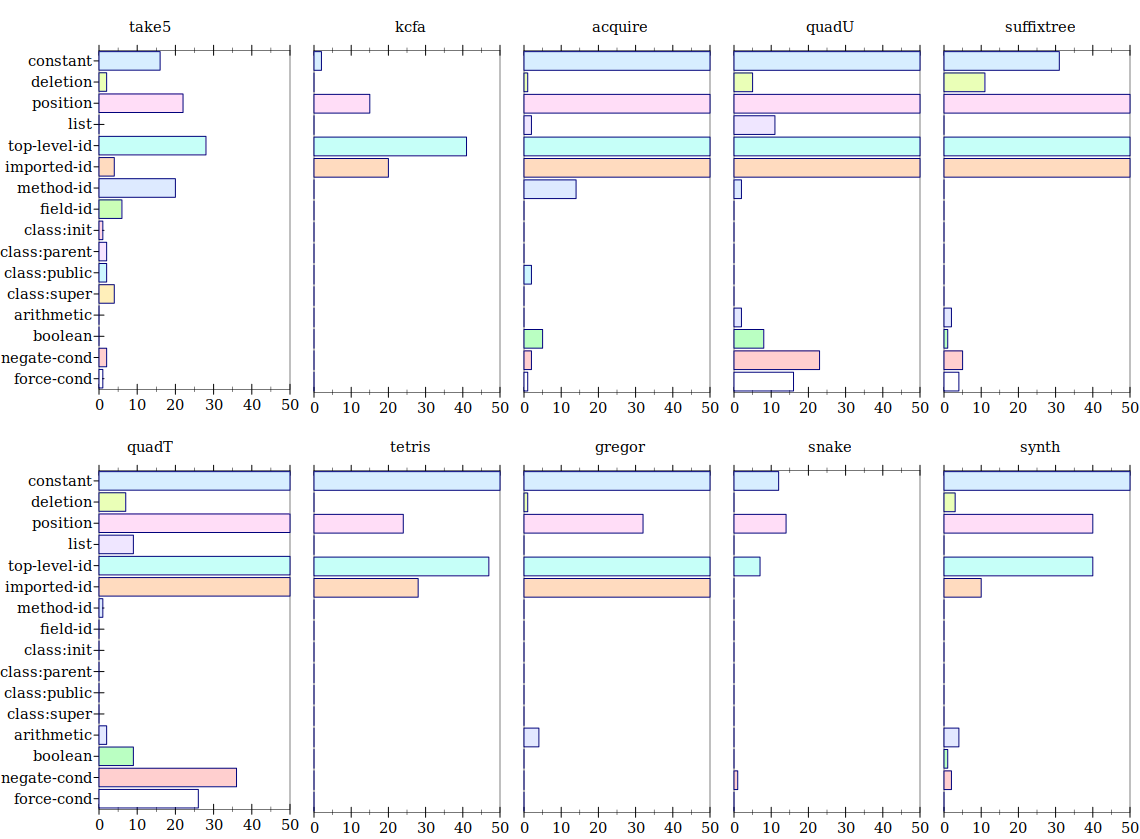
\includegraphics[scale=0.35]{./plots/mutant-breakdown}
  \caption{Interesting debugging scenarios produced by our mutators. Counts are cut off at 50.}
  \label{fig:mutant-breakdown}
\end{figure*}


With the definition of interesting debugging scenarios in hand, we analyze how effective our mutators
are for turning the benchmarks into interesting debugging scenarios.
Indeed the mutators produce at least 72192 interesting debugging scenarios
across all mutants --- there are potentially many more but this is how
many we examined. 
Figure~\ref{fig:mutant-breakdown} breaks down the interesting
debugging scenarios produced  for each benchmark by mutator 
but counts are cut off at 50. The mutators produce at least 40 interesting
scenarios for every benchmark, and these scenarios originate from at
least four different mutators per benchmark.  Thus the mutators result in 
a sizeable and diverse population of scenarios for every benchmark.
Furthermore, every mutator contributes scenarios to at least one
benchmark. Especially some mutators  target specific features of
benchmarks, which
justifies their inclusion. For
instance the class-focused mutators are effective in \texttt{take5}
which jives with the fact that \texttt{take5} is the benchmark with 
the most extensive use of object-oriented features.
